% Asset ID: AS2ForcesTikZ-003
% Source: Chapter 5/7 Forces Transcript
% Related lesson section: Core Theory: Why the second diagram matters
% Purpose: Show the cleaner resolved box diagram.
\documentclass[tikz,border=8pt]{standalone}
\usepackage{amsmath}
\usetikzlibrary{arrows.meta, angles, quotes, decorations.pathmorphing}
\begin{document}
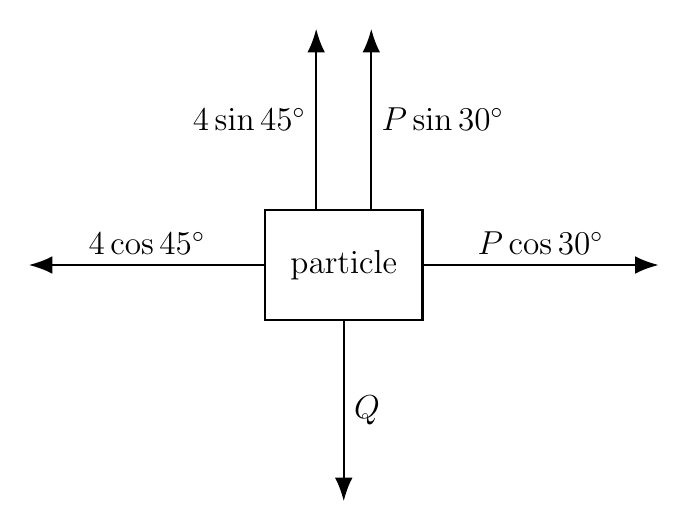
\begin{tikzpicture}[force/.style={-{Latex[length=3mm]}, thick}, comp/.style={-{Latex[length=3mm]}, thick, dashed}, label/.style={font=\large}, note/.style={font=\normalsize}]

\draw[thick] (-1,-0.7) rectangle (1,0.7); \node[label] at (0,0) {particle};
\draw[force] (1,0)--(4,0) node[midway, above,label] {$P\cos30^\circ$};
\draw[force] (-1,0)--(-4,0) node[midway, above,label] {$4\cos45^\circ$};
\draw[force] (-0.35,0.7)--(-0.35,3) node[midway, left,label] {$4\sin45^\circ$};
\draw[force] (0.35,0.7)--(0.35,3) node[midway, right,label] {$P\sin30^\circ$};
\draw[force] (0,-0.7)--(0,-3) node[midway, right,label] {$Q$};
\end{tikzpicture}
\end{document}
